%\begin{savequote}[8cm]
%\textlatin{Jedem Anfang wohnt ein Zauber innne.}
%
%In the core of every beginning lives magic.
%  \qauthor{--- Hermann Hesse's \textit{Stufen}}
%\end{savequote}

\chapter{\label{ch:2-background}Theoretical Background} 

%\minitoc
\section{Introduction}  
This chapter introduces the relevant background for our project and its related work. 
We start by providing an introduction to the field of machine learning, its terminology, and core concepts such as model definitions, objective functions, training methods, and regularisation. The second part of the chapter deals with the specifics of \emph{deep learning} which is a  subfield of machine learning that utilises a certain class of models called \emph{deep neural networks}. We outline different types of neural networks and their respective topologies before discussing concepts like multi-task learning and dropout. The final part of the chapter is dedicated to the problem of counterfactual inference. We motivate the importance of the task and its application areas, and provide a formalisation. Furthermore, we outline the challenges of the problem and different existing approaches that have been applied to it so far. 

%We conclude by relating counterfactual inference to deep learning and describing its open research questions which is the very foundation of this thesis. 

\section{Machine Learning}

\subsection{Motivation}
When conceptualising computer programs, we often think of them as series of discrete, unambiguous, sequential instructions that are executed in a deterministic way and have to be explicitly programmed by a human programmer. 

Many problems --- in particular those for which a well-defined algorithm or effective step-by-step solution strategy exists --- can be successfully expressed and ultimately solved this way. 

Nonetheless, there are domains where this algorithmic approach seems infeasible. A typical example is autonomous driving for which there are almost infinitely many possible situations to consider making it impossible to encode the desired behaviour of an autonomous vehicle as a finite sequence of instructions. 

One potential way to approach these kinds of problems is by using a concept called \emph{machine learning} which is a subfield of computer science that deals with the question of how to teach computer programs to learn to perform a task without being explicitly programmed how to do it. 
% PLAG? Check if this it too close to the quote at wikipedia 

More formally, a common definition of machine learning suggests that an algorithm "is said to learn from experience E with respect to some class of tasks T and performance measure P if its performance at tasks in T, as measured by P, improves with experience E." \cite{ml-definition}
% PLAG?

Transferred to our example of autonomous driving, we could define the task $T$ in terms of "moving the car from an origin A to a destination B" while our performance measure $P$ might include aspects such as the travel time the number of damaged objects or harmed humans. The experience $E$ would represent so called \emph{training data} that is acquired by previously covered distances (either autonomously or by recording the actions of a human driver). 

% TODO Show diagram (model, algorithm, learning, data)

\subsection{Types of Learning}
Machine Learning is typically categorised into three main categories which are briefly outlined in the following. 

\subsubsection{Supervised Learning} 
In a supervised learning setting, the task is to infer a function from a number of samples from a training dataset that is said to be \emph{labelled}. In other words, for each sample in the training data, we have access to the actual function value we want to predict while training the model. 

For instance, we might be interested in predicting housing prices where we are given a dataset consisting of information regarding different properties (e.g. the number of rooms and the area in $m^2$), commonly referred  to as \emph{features} or \emph{covariates}, and the actual price for which the house has been sold, called \emph{outcome}, \emph{target}, or \emph{label}. 

Once the \emph{model has been trained} --- i.e. we have found the parameters of an appropriate function that best describes the historic dataset --- we can use the same model to predict the housing prices for unseen data points. 

Such a task of predicting a continuous variable is often referred to as a \emph{regression problem} whereas the prediction of a discrete output is called a \emph{classification problem}. 

\subsubsection{Unsupervised Learning} 
In contrast to supervised learning, the training set of an unsupervised learning problem does not contain the target labels. Typical tasks in this setting include inferring structural patterns from the data and \emph{clustering }it accordingly. 

It is important to note that for supervised learning, there is normally no concept of an underlying \emph{ground-truth} that we are trying to predict. In other words, the performance (or quality) of the outcome typically cannot be measured or defined in absolute terms but depends on the domain-specific use-case of the clustering. 

Another important task in unsupervised learning is \emph{dimensionality reduction} for which a high-dimensional dataset is reduced to a target lower dimension while simultaneously trying to minimise the information loss. 

\subsubsection{Reinforcement Learning}
In reinforcement learning, a software agent has to learn a sequence of appropriate actions in a dynamic environment in which the consequences of an action might not be immediately accessible but accumulate to a long-term reward that ought to be maximised. \cite{reinforcement-learning}

A most prominent example was mentioned earlier with the task of autonomous driving in which a vehicle is governed by a piece of software that has to find an adequate series of actions (i.e. steering and regulating speed) in order to reach a target destination in a complex and dynamically changing environment. 

\subsection{Machine Learning Models}
% GRAPH Re-create graph!
\begin{figure}[h]
	\caption{Schematic Approach of Machine Learning. A selected model $M$ is trained on a dataset $D$ using a learning algorithm $A$.} \label{fig:machine-learning-approach}
	\centering
	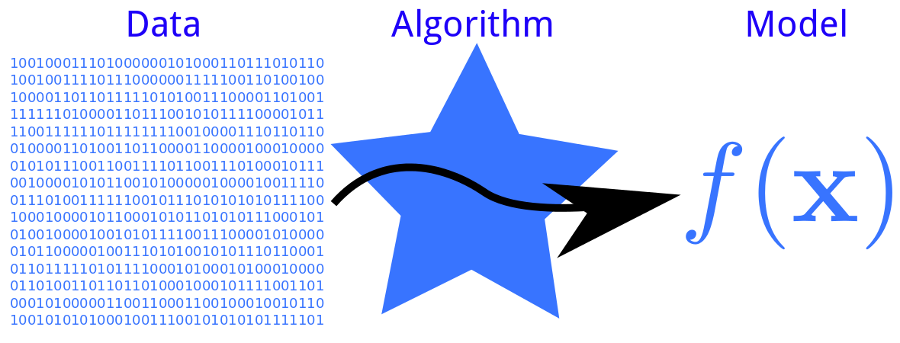
\includegraphics[width=0.5\textwidth]{figures/chapter-2/machine-learning-approach.png}
\end{figure} 

Machine learning is based on the concept of selecting an appropriate model and fitting it to a given (training) data set using a training algorithm illustrated in figure \ref{fig:machine-learning-approach}. 

For instance, we might want to use a \emph{linear model} $f$ for our task of predicting housing prices
\begin{equation}
f_{\mathbf{w}, b}(\mathbf{x}) = \mathbf{w}\cdot \mathbf{x} + b,
\end{equation}
where $\mathbf{x}$ corresponds to the input vector containing the features of the house, and $\mathbf{w}, b$ represent the parameters of our linear model commonly referred to as \emph{weights} and \emph{bias}. We can then make use \emph{linear regression} to fit our linear model to our labelled dataset of existing houses and their prices. 

The selection of an appropriate model is of great importance and determines factors such as the trade-off between the expressiveness or \emph{variance} of the model (i.e. its ability to capture complex relationships) and its potential to generalise to unseen data points. Additionally,  computational considerations such as time and space complexity of the model and its training process have to be taken into account. 

Consequently, the selection of an appropriate model typically depends on the task, the training datasets, and its characteristics. Typical alternatives to the linear model include \emph{support vector machines}, \emph{decision trees}, and \emph{neural networks}. 
% TODO What are other typical models. How do they compare against each other? 
% Should I sketch them out here? 

This dissertation focuses on using \emph{deep learning} for the problem of counterfactual inference. Therefore, a dedicated part of this chapter deals exclusively with deep neural networks and describes their characteristics in more detail. 


\subsection{Variance, Bias, and Regularisation} \label{sec:regularisation}
% GRAPH Re-create graph!
\begin{figure}[]
	\centering
	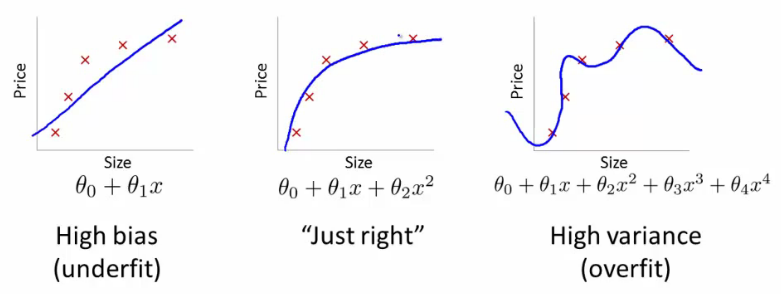
\includegraphics[width=0.8\textwidth]{figures/chapter-2/overfitting-underfitting.png}
	\caption{Visualisation of Bias variance Tradeoff. The model on the left is ... whereas the middle one ... and the right one is ...}	\label{fig:overfitting-underfitting}
\end{figure}
When training our model we have to find the right balance between fitting it most accurately to the training data while making sure that it still generalises well to unseen data points. This consideration is commonly referred to as \emph{trade-off between bias and variance},  illustrated in figure \ref{fig:overfitting-underfitting}. 

The model on the left tries to fit a straight line to a dataset which expresses polynomial properties resulting in a poor approximation often referred to as \emph{underfitting}. We might say the model has a high \emph{bias} and is therefore too simple to accurately describe the relationship in the data. 

In contrast, the model on the right uses high-order polynomial features and is able to perfectly fit the data resulting in a training error of zero. This, however, is typically not desired as we would merely "memorise" the training data and perform poorly on any unseen future data points. In other words, we are \emph{overfitting} the training dataset because of a \emph{high variance}.  

Consequently, the objective is to train a model that neither overfits nor underfits the training data and generalises well to unseen datapoints ( illustrated by the model in the middle). 

The most common approach to achieve this is by selecting a model which is likely to have a sufficient variance to capture the complexity of the data (thus avoiding underfitting) and then making use of a concept called \emph{regularisation} to avoid overfitting. 

Regularisation can be achieved by introducing a \emph{regularisation term} in the objective function that imposes a penalty for learning models that are too complex. Consider the terms 
\begin{align} 
R_{l1}(\mathbf{w}) = \sum_{i=1}^{d}  \lvert \mathbf{w}_i \lvert  && \text{and} &&R_{l2}(\mathbf{w}) = \sum_{i=1}^{d}  \mathbf{w}_i^2,
\end{align} 

where $d$ refers to the dimension of the weights parameter $\mathbf{w}$, that both penalise the sum of the weights (in terms of the absolute value or as a quadratic function, respectively). This way, we ensure that the model learns the parameters in a way that only attaches high weights to highly predictive features since their gain has to outweigh the penalty imposed by the regularisation term. 
 
We will cover the concept of regularisation in more detail in section \ref{sec:dropout} for neural networks as they represent the class of models that this thesis is focus on. 


%When using a complex model with a high variance, we might naively fit our model to the training data perfectly, resulting in a training error of zero. This, however, would merely "memorise" the training data and might perform poorly on unseen future data points. This phenomenon where we overfit the training data is often referred to as \emph{high variance}. 
%In contrast, if the model is too simple, we night not be able to accurately capture the relationship in our data leading to equally poor results. In this case, we are under-fitting the data and our model has a so called \emph{high bias}.
%
%


% TODO Should I include learning curves as well? 
%% TODO! Re-create graph!
%\begin{figure}[]
%	\label{fig:machine-learning-approach}
%	\caption{Visualisation of Learning Curves. The left model is ... whereas the right model is ...}
%	\centering
%	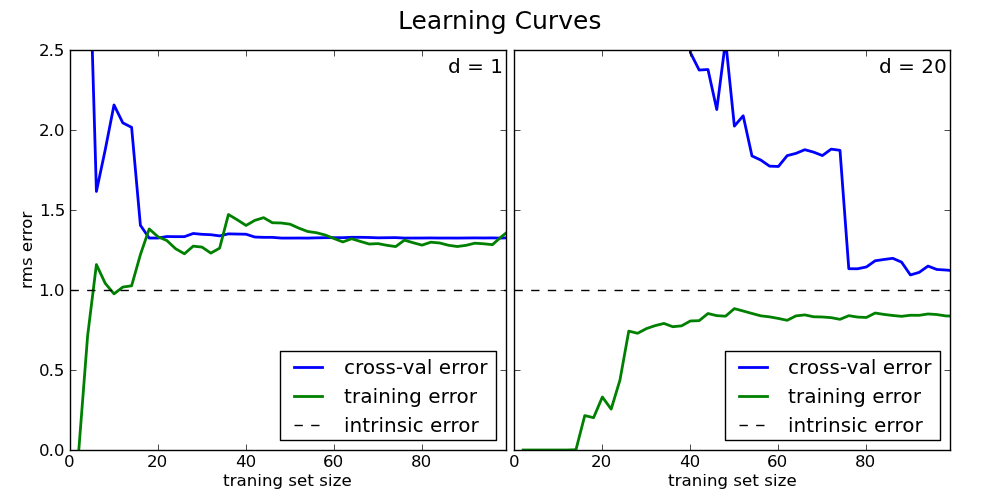
\includegraphics[width=0.8\textwidth]{figures/chapter-2/learning-curves.png}
%\end{figure}




\section{Deep Learning}
\subsection{Introduction}
Deep learning refers to a field of machine learning that is based on the use of so called \emph{deep neural networks}. 

The approach is loosely inspired by how the human brain works,  modelling biological neurons and their interconnections in terms of artificial neurons that express similar properties.


\paragraph{Biological Foundations}
The details about our understanding of the mechanics and biochemical processes of the human brain are well beyond the scope of this thesis. On a conceptual level, however, each neuron receives inputs signals on its dendrites which are connected to the axons of neighbouring neurons. The input signals are accumulated and processed within the cell body causing the cell to output a signal on its own axon (in turn representing a potential input for other cells). By means of these interconnections, the neurons form a highly complex structure that can be conceptualised in terms of a biological neural network. It is estimated that the human brain contains about 100 billion neurons  allowing it to process complex signals and reason about abstract concepts \cite{number-of-neurons}. 
% TODO What about learning? 

In a bionic fashion, an \emph{artificial neural network} (henceforth called \emph{neural network}), adopts this architecture in a simplified way by defining a network of \emph{artificial neurons} (discussed in details in section \ref{sec:mlp}) that are connected according to a certain topology. The analogy between the human and the artificial neurons is illustrated in figure \ref{fig:artificial-neuron}: The artificial neuron receives input signals, processes the signals according to an internal activation function, and outputs a computed signal on its own. 

Analogous to its biological counterpart the a neural network is able to capture complex non-linear relationships to approximate arbitrarily complex functions. 



% GRAPH Recreate graph
\begin{figure}[h]
	\caption{A biological neuron vs. an artificial neuron}\label{fig:biological-vs-artificial-neuron}
	\centering
	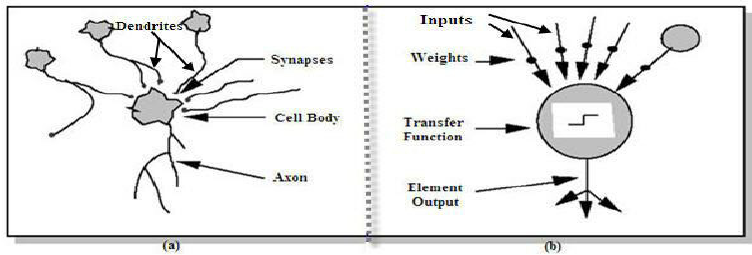
\includegraphics[width=0.8\textwidth]{figures/chapter-2/biological-vs-artificial-neurons.png}
\end{figure}


\paragraph{History of Neural Networks}The theoretical foundations of neural networks date back to the 1940s \cite{nn-history}, before becoming popular in the 1970s after the \emph{backpropagation algorithm} (see section \ref{sec:training}) had been successfully applied to neural networks  \cite{backprop1}. Following an initial enthusiasm, however, neural networks fell out of favour in the following decades due to the realisation that the models typically expressed a degree of computational complexity that could not be accommodated by the existing hardware.

This changed again in the early 2010s when a neural networks significantly outperformed existing methods in a variety of fields such as computer vision \cite{imagenet} and natural language processing \cite{nlp}. % CITE imagenet

Ever since, deep neural networks have been responsible for some of the most recent successes in machine learning, including self-driving cars and defeating human champions in the game of Go \cite{alphago}.
The renaissance of neural networks and its recent successes have typically been attributed to two key factors: Firstly, the advancements in computational capabilities on modern GPUs and other highly-optimised processing units such as \emph{FPGAs} and \emph{ASICS}.
Secondly, the widespread availability of large datasets that can be used for training the models such as web-scale text corpora for natural language processing or large databases of images that can be used in computer vision. 

\paragraph{Status Quo} Today, deep neural networks represent the state-of-the-art for many problems. They are widely considered one of the most promising areas of machine learning and artificial intelligence in general and have received a high level of attention in society, media, and politics. Nevertheless, the usage of deep neural networks poses a multitude of computational, architectural, and domain-specific questions that are the subject of ongoing research. 

\subsection{The Multilayer Perceptron} \label{sec:mlp}
In order to understand how neural networks work, we first investigate one of its most basic forms: the \emph{multilayer perceptron} or MLP. 

% GRAPH Redo graph
\begin{figure}[H]
% GRAPH-LABEL Add proper description
\centering
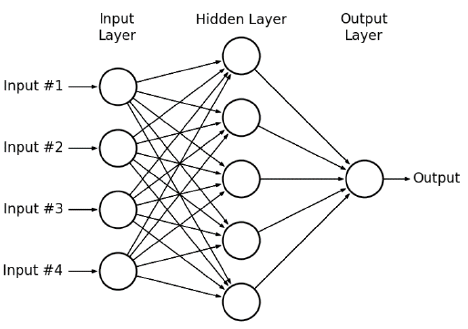
\includegraphics[width=0.7\textwidth]{figures/chapter-2/multilayer-perceptron.png}
\caption{Prototypical multilayer perceptron with a single hidden layer.}\label{fig:multilayer-perceptron}
\end{figure}
Figure \ref{fig:multilayer-perceptron} depicts the schematics of a MLP. As the name suggests, it consists of multiple layers each containing a fixed number of artificial neurons (henceforth called neurons) that are interconnected exclusively by neurons of neighbouring layers. The first, so called \emph{input layer}, is followed by one or more \emph{hidden layers} leading to a final so called \emph{output layer}. 

\begin{figure}[h]
	\centering
	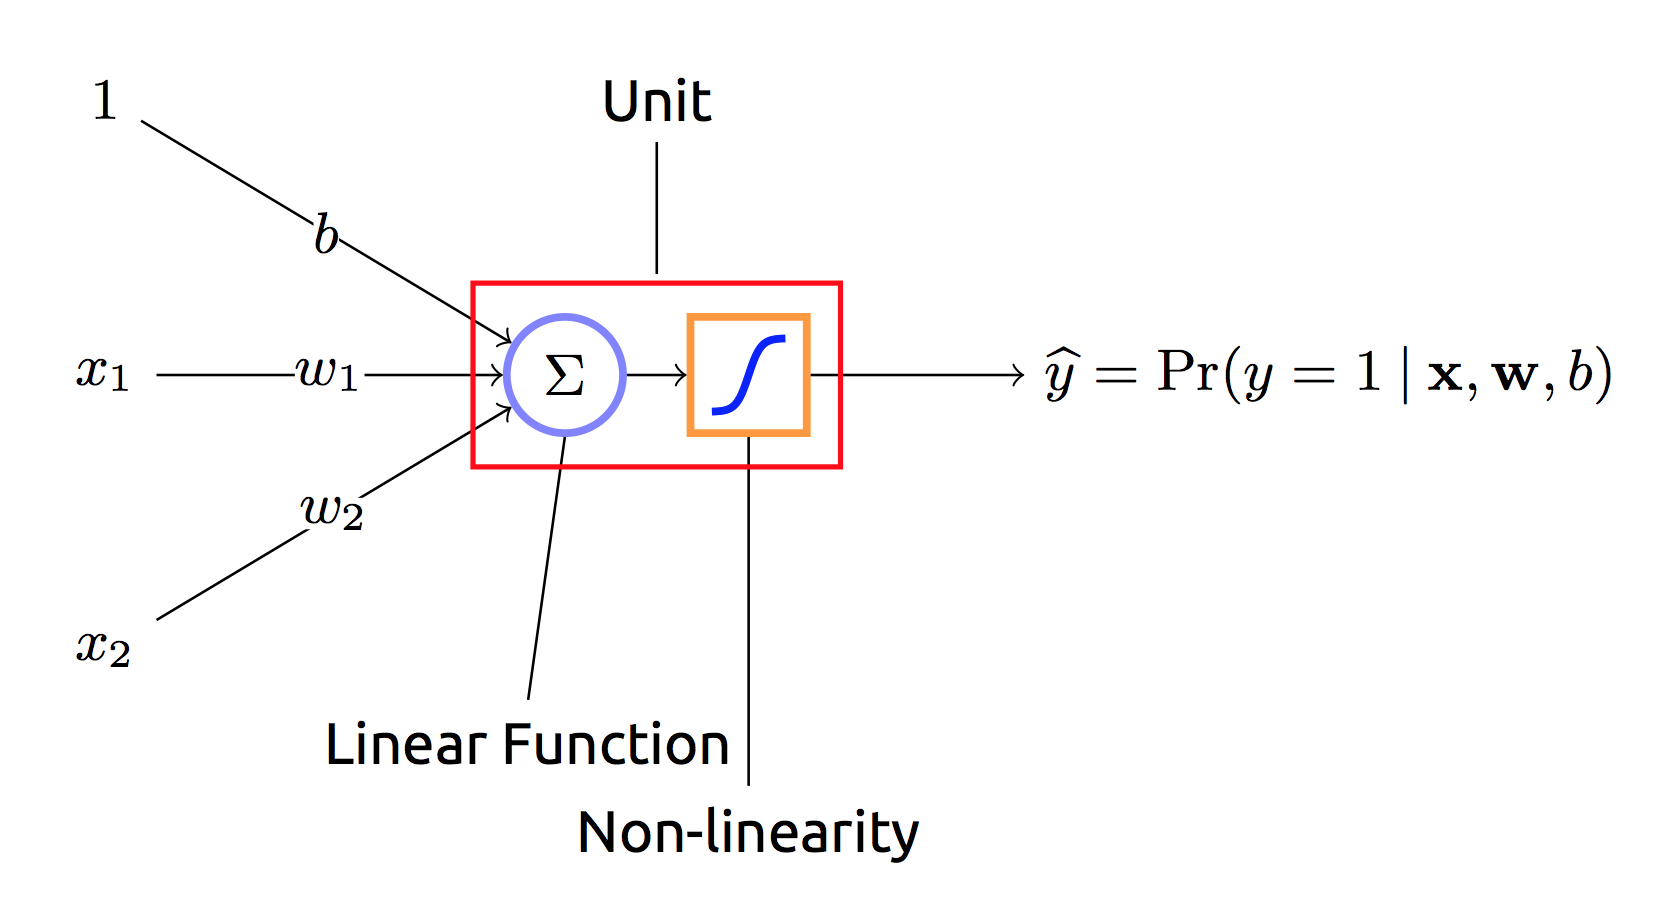
\includegraphics[width=0.6\textwidth]{figures/chapter-2/artificial-neuron.png}
	\caption{Basic building block: Artificial Neuron used for classification.}\label{fig:artificial-neuron}   
\end{figure}

In a MLP, the basic building block is the artificial neuron or \emph{unit} which is illustrated in figure \ref{fig:artificial-neuron}. 

Its output $y$ is computed as 
\begin{equation}
	% MATHS Check, looks weird with b in front
	y = \phi(b + \sum_{i=1}^{n} w_i x_i)
\end{equation}
where $x_1, \ldots, x_n \in \mathbb{R}$ corresponds to the inputs of the neuron, $w_1, \dots, w_n\in \mathbb{R}$ to the weights and $b \in \mathbb{R}$ to a bias ($w$ and  $b$ are the parameters of the model that ought to be learnt) and $\phi: \mathbb{R} \rightarrow \mathbb{R}$ to a non-linear function referred to as \emph{activation function}. Typical choices for $\phi$ include 
\begin{align*} 
\phi(x) = \sigma(x) = \frac{1}{1 + e^{-x}} && \text{or} && \phi(x) = tanh(x) = \frac{1  - e^{-2x}}{1  + e^{-2x}}
\end{align*} 
where $\sigma(x)$ refers to the \emph{sigmoid function}, $tanh(x)$ to the \emph{hyperbolic tangent}, and $ReLU$ to \emph{rectified linear unit}. While each of these activation functions has different properties as illustrated in figure \ref{fig:activation-functions}, a typical characteristic is that they map the input value to the closed interval $[0, 1]$. 

% GRAPH Add plots for sigmoid, tnah, and relu
\begin{figure}[h]
	\caption{Typical Activation functions}\label{fig:activation-functions}   
	\centering
	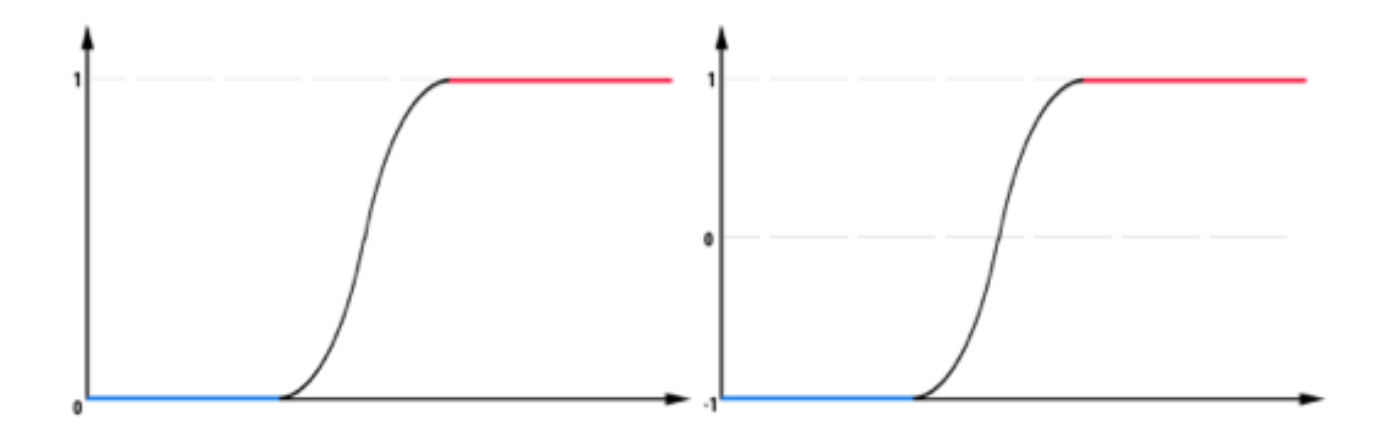
\includegraphics[width=0.6\textwidth]{figures/chapter-2/activation-functions.png}
\end{figure}


% TODO What else do I need to write about MLPs?  Equations for the outcome? 
%Given this definition of a single unit, the final value $y$ of the outcome layer can be formalised as the concatenation of the different activation functions forward-propagated from the input layer to the output layer. For the MLP depicted in figure \ref{fig:multilayer-perceptron}, this means.
%
%\begin{align}
%x = 
%\end{align}

Despite the relative simplicity of this model, it can be shown that a MLP with a single hidden layer and an activation function as defined above is able to represent any arbitrarily complex non-linear function \cite{mlp-power}.

\subsection{Types of Neural Networks} \label{sec:nn-types}
There are different types of neural networks defined by a number of characteristics such as their topology and the direction of information flow. 

\paragraph{Feed-Forward Neural Networks} Closely related to the MLP described in the previous section, feed-forward neural networks (FFNNs) represent a class of networks that is characterised by a set of hidden layers that have a similar shape and are often fully connected (i.e. every node in the hidden layer $L_i$ is connected to every node in layers $L_{i-1}$ and $L_{i+1}$). As the name suggest, the information flow is uni-directional from the input layer through the hidden layers to the output layer. These networks represent the most general type, making no assumptions about the input data and can be used for regression and classification tasks alike (the difference often lies exclusively in the lack of a non-linear activation function in the output layer of classification tasks).

\paragraph{Convolutional Neural Networks} While FFNNs make no assumptions about the input data whatsoever, it is often useful to exploit domain-specific knowledge about the specific input data. For instance, in computer vision the input of a network is typically an image encoded as pixmap with the intensity values of each pixel. In this case, it seems naive and inefficient to assume independence of the inputs ignoring aspects like the principle of locality of neighbouring pixels which are more likely to have a similar colour or intensity than two randomly-selected pixels. 
\begin{figure}[h]
	\centering
	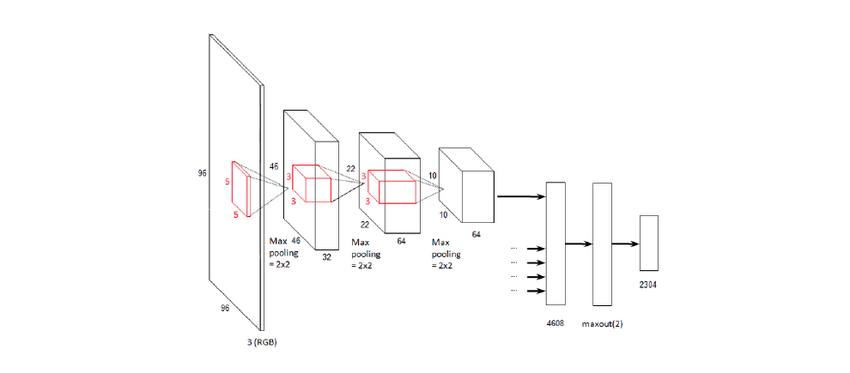
\includegraphics[width=1\textwidth]{figures/chapter-2/convnet.png}
	\caption{Convolutional Neural Network}\label{fig:convnet}   
\end{figure}
A convolutional neural network or \emph{convnet} (illustrated in figure \ref{fig:convnet})is a special kind of feed-forward neural network whose architecture is designed to exploit the principle of locality in the data. This is normally achieved by alternating \emph{convolutional layers} and \emph{pooling layers}. The convolutional layers run a filter or \emph{kernel} across the their input layer which performs an image convolution and can be thought of a way to detect features (such as edges) in the image. The pooling layers usually perform an aggregation (such as taking the maximum of multiple values) over the previous layer to reduce its dimensionality on focus on the salient features.  

While convnets are particularly useful in computer vision and represent the state-of-the-art, for instance, in image classification, they can also be applied in other fields in which the data expresses some principle of locality such as natural language processing. 

\paragraph{Recurrent Neural Networks} In contrast to FFNNs and convnets for which the information flow is strictly uni-directional, recurrent neural networks (RNNs) are characterised by the existence of feedback loops that allows the outputs of a unit in layer $L_i$ to be process as input by any other layer $L_j$, even if $i \geq j$.

This allows the network to learn and store an internal state which can be conceptualised as memory. Such a memory enables the network to effectively deal with sequences of data such as time-series values, natural language, or even acoustic signals like music. 

\begin{wrapfigure}{r}{0.5\textwidth}
	\centering
	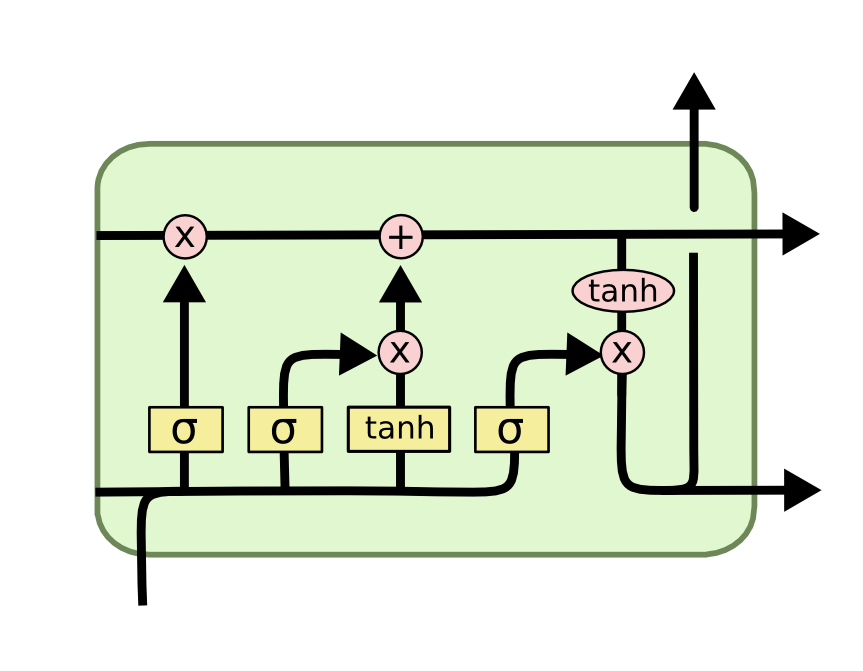
\includegraphics[width=0.5\textwidth]{figures/chapter-2/lstm.png}
	\caption{LSTM}\label{fig:lstm}   
\end{wrapfigure}

In spite of the benefits the recurrent architecture of the network provides, it also introduces a number of computational challenges such as the so called \emph{vanishing gradient problem} which stems from the additional distance the gradient is backpropagated (see next section % TODO Reconsider training section. Should it come before? 
) through the computation graph of the network. In order to circumvent this problem, a number architectures has been proposed for individual cells within the RNN, most notably \emph{long short-term memory} (LSTM) cells and \emph{gated recurrent units} (GRUs). Since RNNs are not of primary interest for the models we investigate for counterfactual inference, the detailed mechanics for these cells are outside the scope of this dissertation.  On a conceptual level, however, LSTM cells address the vanishing gradient problem by utilising a number of \emph{gates} (as illustrated in figure \ref{fig:lstm}) that allow the cell control how the gradient is propagated through the cells, effectively allowing it to decide when to store and when to reset (i.e. forget) its internal state.

Today for many problems in machine learning, RNNs represent the state-of-the-art when dealing with sequential data such as natural language and time-series. 

\subsection{Training}\label{sec:training}
Training a neural network refers to the process of fitting the parameters of the model (i.e. the weights and biases for each cell) to the training data with respect to a given objective function. 

\paragraph{Objective Function}
\begin{wrapfigure}{r}{0.4\textwidth}
	\centering
	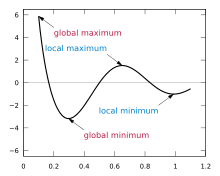
\includegraphics[width=0.4\textwidth]{figures/chapter-2/local-minima.png}
	\caption{Local Minima}\label{fig:local-minima}   
\end{wrapfigure}

The objective function (also called \emph{loss function} or \emph{error function}) defines a performance metric for the model. It is the goal of the training procedure to infer appropriate parameters for the model that maximise its performance (i.e. minimise its loss). 

Figure \ref{fig:local-minima} illustrates this concept by depicting the graph of an objective function $f$ that takes a one-dimensional input (real numbered scalar). As we can see, the function possesses multiple extreme values -- in particular one local minimum at $x = ?$% TODO add proper position
and a global minimum at $x = ?$. % TODO add proper position.  % IMPORTANT!!! GRAPH Add the appropriate positions


In cases where an algebraically obtained closed-form solution for the minimum is not feasible or too computationally expensive, the minimum is often obtained by optimisation algorithms (see below). Since these algorithms often operate in a \emph{greedy} manner, i.e. by a applying series of local operations that has no knowledge about the global surface of the function, we are facing the potential problem of only finding a local optimum but missing out the global one. As a consequence, it is desirable to use convex objective functions that, by definition, only have one (global) optimum. 

The actual loss function is dependent on the problem task and can be derived by a maximum likelihood estimation (MLE). For regression tasks, a common choice is the mean squared error between the prediction $\hat{Y}$ and the actual output value $Y$ defined as 


\begin{align} 
L_{MSE}(w,b) = \frac{1}{n} \sum_{i=1}^{n}(\hat{Y}_i - Y_i)^2.
\end{align} 
For (binary) classification problems we typically use the cross-entropy
\begin{equation}
	L_{CE}(w,b) = - \frac{1}{n} \sum_{i=1}^{n} (Y_i \log \hat{Y}_i + (1 - Y_i) \log 
	(1- \hat{Y}_i)
\end{equation}
as loss function. 

\paragraph{Gradient Descent} We typically make use of an optimisation algorithm that tries to minimise the output of our loss function by capturing to what extend our predictions differ from the target values. A widely used example is \emph{gradient descent} which is an iterative optimisation algorithm that can be used to find a minimum value of a function. Gradient descent repeatedly computes the gradient of the loss function at the current position and subtracts a proportion of the gradient from it until the gradient converges towards zero (which is the case at a minimum) or a stopping condition is satisfied. Intuitively, the subtraction of the gradient can be conceptualised by taking iterative steps in the direction of the steepest descent until a minimum value is reached. 
Formally, we are looking for $x = \text{argmin} f(x)$ by iteratively computing

\begin{equation}	
	\label{eq:gradient-descent-update}
	x_{n+1} = x_n - \alpha \cdot \nabla f(x_n),
\end{equation}
where $x_i$ refers to our position at iteration $i$ and $\alpha \in \mathbb{R}^+$ is a parameter called the \emph{learning rate} that defines the step size of our descent. Choosing an appropriate learning rate expresses a trade-off between reducing the number of required iterations (high learning rate) and a making sure the function converges and does not "overshoot" the actual minimum $x^*$ causing the algorithm to potentially oscillate around the desired optimum. Consequently, it is often desirable to use an \emph{adaptive learning rate} instead, i.e. making $\alpha: \mathbb{N} \rightarrow \mathbb{R}^+$ a function dependent on the current iteration $i$. 

There two main types of gradient descent: \emph{batch gradient descent} computes the gradient for entire dataset before applying an update rule as defined in equation \ref{eq:gradient-descent-update} which is most exact but computationally expensive as the algorithm has to iterate through all $n$ data points in the dataset before applying a single update. In contrast, \emph{stochastic gradient descent} computes the gradient of a random (hence the name) sample and applies an update according to this sample alone which is less computationally expensive. The choice between batch gradient descend and stochastic gradient descend therefore represents a trade-off between accuracy and computational costs. In addition to this dichotomy, there exists a hybrid variation called \emph{minibatch gradient descent} which computes the gradient on a batch which is a subset of the entire dataset. 

\paragraph{Backpropagation} For gradient-based optimisation algorithms it is mandatory to compute the partial derivatives of the objective function $L$ with respect to any weight $w$ or bias $b$ in the neural network that needs to be learnt. In a deep neural network with multiple hidden layers this can be a complex task as the change of a weight influences the outcome (and therefore the loss function) only indirectly by propagating its change through subsequent layers. 

The \emph{backpropagation algorithm} \cite{backprop1} introduces an efficient method to compute the partial derivatives. It conceptualised the network as a concatenation of functions and is based on the simple idea of repeatedly applying the \emph{chain rule} known from calculus to compute the partial derivatives with respect to each parameter (weights and biases) of interest. 

%\begin{wrapfigure}{r}{0.6\textwidth}
%	\centering
%	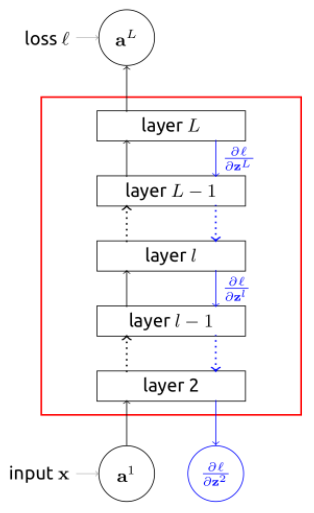
\includegraphics[width=0.6\textwidth]{figures/chapter-2/backpropagation.png}
%		\caption{Backpropagation}\label{fig:backpropagation}   
%\end{wrapfigure}
\begin{figure}[h]
	\centering
	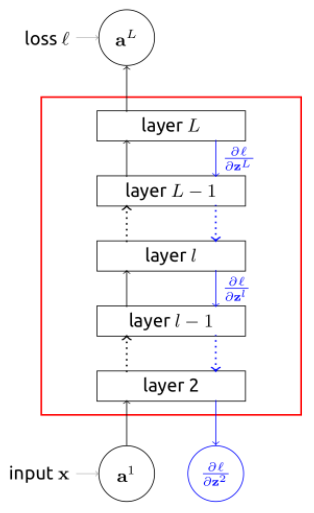
\includegraphics[height=0.5\textwidth]{figures/chapter-2/backpropagation.png}
	\caption{Backpropagation}\label{fig:backpropagation}   
\end{figure}


The training is then executed in two alternating phases that are illustrated in figure \ref{fig:backpropagation}: In the \emph{forward pass} the inputs are propagated through the network from the input layer through the hidden layers until a predicted outcome $\hat{Y}$ is available in the output layer. Using the predicted outcome $\hat{Y}_i$, the actual outcome $Y_i$, and the loss function $L$ we are able to compute a loss \emph{l}.
In the second phase -- the \emph{backward pass} the partial derivatives are computed for the weights and biases of each unit all the way back until the first layer after the input layer. 

Once the partial derivatives are computed, we can update each parameter according to our optimisation algorithm, for instance by applying the update rule defined in equation \ref{eq:gradient-descent-update}. 
The backpropagation algorithm therefore represents an effective technique to compute the gradient of the loss function with respect to the different parameters and is considered an essential part of the training of neural networks. 


\subsection{Dropout} \label{sec:dropout}
As described in section \ref{sec:regularisation}, regularisation is an important concept in machine learning in order to avoid overfitting the training data. While in theory, a traditional approach like \emph{l1} (lasso) and \emph{l2} (weight-decay) regularisation are conceivable, a number of regularisation techniques have been proposed that are specific to the mechanics of neural networks. 

One of the most-used approaches is called \emph{dropout} and was proposed by \citedate{dropout} in 2014. The basic idea is that during training every neuron is kept active only with a certain probability $p$. Conversely, with a probability of $1-p$ it is masked out and represents an output of zero. Intuitively, this prevents the network from becoming too dependent on a particular neuron as it is forced to learn an alternative representation when the neuron is disabled. As a consequence, the network learns a representation that generalises better giving dropout a regularising influence on the network. Similar to the regularisation hyper-parameter $\lambda$ described earlier, the dropout probability $p$ represents a hyper-parameter that has to be chosen appropriately.
\begin{figure}[h]
	\centering
	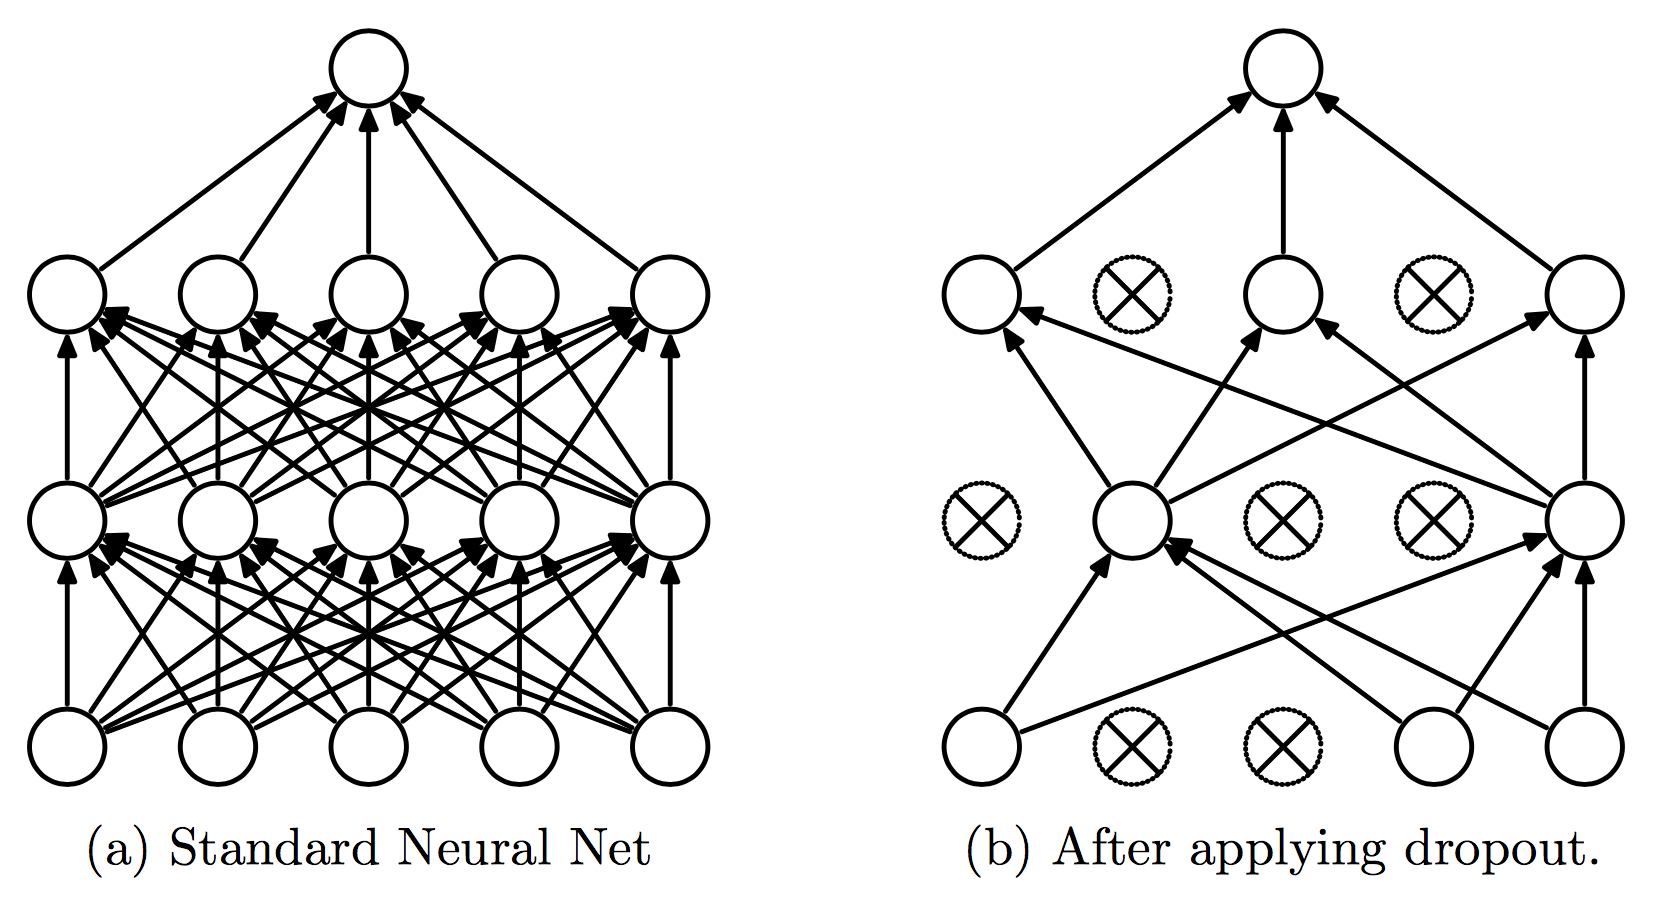
\includegraphics[width=0.8\textwidth]{figures/chapter-2/dropout.png}
		\caption{Dropout}\label{fig:dropout}
\end{figure}


Figure \ref{fig:dropout} illustrates this the concept of dropout: The original network (left side) is thinned out by the dropout resulting in the network on the right side. 

Today, dropout represents the de-facto standard for regularising neural networks and preventing them from overfitting. 


\subsection{Multi-Task Learning}
Neural networks are typically used to perform a single task that is formalised by minimising an appropriate objective function. However, sometimes it is desirable to train the network on multiple (related) tasks simultaneously. 

% GRAPH Cite Hinton % CITE Sebastian Ruder
\begin{wrapfigure}{r}{0.4\textwidth}
	\caption{Multi-Task Learning}\label{fig:multitask-learning}   
	\centering
	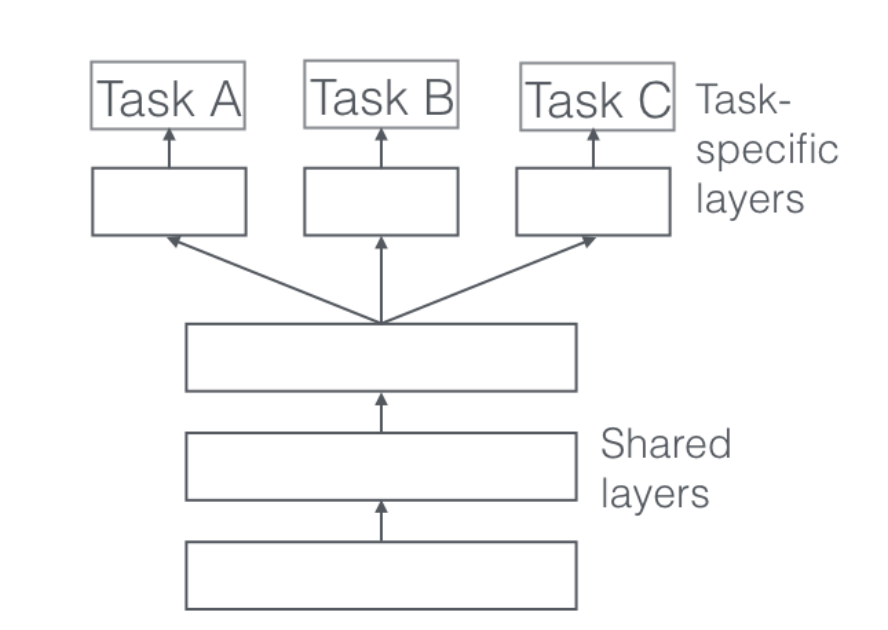
\includegraphics[width=0.4\textwidth]{figures/chapter-2/multitask-learning.png}
\end{wrapfigure}
As illustrated in figure \ref{fig:multitask-learning}, such a multi-task neural network is characterised by a number of layers that are shared between all tasks and a number of layers that are task-specific. Each task typically provides its own objective function which is optimised jointly with the objective functions of the other tasks. 

Multi-task learning can have a variety of desirable properties: Firstly, multi-task neural networks are typically less prone to overfitting as the shared layers have a regularising effect on the network forcing it to learn a shared representation among all tasks. Moreover, they allow influencing the way a task is learnt on a fine-grained level by introducing inductive biases \cite{inductive-bias} that are provided by the other tasks. This means that we can make a primary task more inclined towards considering related sub-tasks. 

As an example for multi-task learning, we consider training a spam classifier for emails. Different users might have distinct distributions over the features of emails they receive due to factors such as language, age, and their interests. Therefore, we can conceptualise the individual classifiers as a number of different tasks. Despite their differences these tasks are highly related allowing us to treat the classifier as a multitask-learning problem. Ideally, the shared layers would learn common concepts of the characteristics of spam emails whereas the individual task-specific layers would take into account the specific characteristics of the user. 

% ... "Bias-free learning is impossible; much of the power of an inductive learner follows directly from the power of its inductive bias [Mitchell 1980]."

% CITE Sebastian Ruder
% CITE http://www.cs.cornell.edu/~caruana/mlj97.pdf




\subsection{Model Selection and Architecture Learning} 
In section \ref{sec:nn-types} we introduced the main types of neural networks, each suitable for different kinds of tasks. However, even after selecting a specific type, there are still a number of architectural considerations that influence the performance of the model. These considerations represent model-level hyper-parameters that are normally defined a-priori and have to be chosen in addition to the hyper-parameters that we already discussed in the previous sections (i.e. the learning rate $\alpha$, the dropout probability $p$, and the type of activation function $\phi$). The following lists such model-level hyper-parameters and how they might affect the network. 

\subsubsection{Model Hyperparameters}
\paragraph{i) Number of layers} The number of layers (or \emph{depth}) of the network is a key design decision for the model's architecture and greatly influences its performance. In general, a greater number of layer results in a more complex model with higher variance increasing its ability to capture complex non-linear dependencies. On the flip side, % TODO Can I say this? 
it also increases the risk of  over-fitting the training data and therefore requires stronger regularisation. From a practical perspective, a higher number of layers also causes the model to be more computationally expensive and require a larger memory to store the trained parameters. 

Consequently, the number of layers corresponds to the classical trade-off between bias and variance discussed in section \ref{sec:regularisation} and thus depends on the amount of available data, the degree of regularisation, and computational considerations. 


\paragraph{ii) Number of units per layer} In addition to the number of hidden layers, we need to decide on an appropriate number of units per hidden layer (network \emph{width}). The decision follows a similar rationale to the number of layers: A high number of units per layer increases the variance of the model allowing it to accommodate more complexity while increasing the risk of over-fitting.  


\subsubsection{Hyper-Parameter Optimisation} \label{sec:hyper-param-optimisation}
In contrast to ordinary parameters (i.e. weights and biases) of the model, hyper-parameters are typically not learnt during training but need to be chosen a-priori. However, there are three main techniques for deriving suitable hyper-parameters:

\paragraph{i) Grid Search} The most basic form of finding appropriate hyper-parameters is to perform a \emph{grid search}. This means iteratively trying a set of candidate values for each hyper-parameter leading to an exhausting search over the space of potential hyper-parameters. After each iteration, the model is trained and then evaluated on a dedicated \emph{cross validation set} which is a subset of the entire dataset disjoint from the training and test set. The set of hyper-parameters with the maximum performance is ultimately chosen for the model.   
While this approach is feasible for a small search space, it becomes computationally challenging if the space of potential hyper-parameters is large. 

\paragraph{ii) Random Search} An alternative to grid search that is computationally less expensive is \emph{random search}: Instead of trying every possible hyper-parameter in the search space exhaustively, this approach randomly samples hyper-parameters from the search space a fixed amount of times. 

\paragraph{iii) Bayesian Optimisation} Bayesian optimisation \cite{bayesian-optimisation} of hyper-parameters uses \emph{Gaussian processes} (GPs) to map a distribution over the hyper-parameters to an (initially unknown) objective function of our model that we want to optimise. We are trying to evaluate the search space of hyper-parameters in a way, that provides the maximum insight about the objective function and its potential minimum.  This is achieved by using concepts of Bayesian inference, i.e. obtaining a \emph{posterior probability} by updating our previous beliefs (\emph{prior}) with evidence following \emph{Bayes' Rule}. 

In practice, it has been shown that Bayesian optimisation has the potential to outperform competing approaches (such as grid search) while requiring a fewer number of iterations \cite{bayesian-optimisation-results}. Nevertheless, due to the curse of dimensionality, in most settings the process is still considered computationally expensive. 


%\subsubsection{Architecture Learning}
%Nevertheless, a number of approaches to automatically deriving suitable architectures has been proposed by a concept called 
%
%It is difficult to derive proper architecture. 
%What's the right number of hidden layers? What's the right number of hidden units per layer, etc? 
%Different approaches to architecture learning. Optimal Brain Surgeon/Damage. GridSearch, RandomSearch, Bayesian Optimisation.

%\subsection{Challenges}
%Computational complexity
%Lots of parameters (high memory)
%Lots of hyper-parameters 
%Low Understandability. Some people confuse softmax with confidence. 
%
%Lorem ipsum dolor sit amet consectetur, adipiscing elit mus neque montes, suspendisse et sociis vestibulum.

\section{Counterfactual Inference} \label{sec:counterfactual-inference}

\subsection{Motivation}
% TODO Check overlap with Introduction section
The concept of causality represents the foundation of disciplines such as reasoning and logic. To some extent, most scientific research can be considered as an attempt to investigate the causal relations within different concepts in order to understand what \emph{cause of actions} results in  what \emph{effect}.

Despite its importance, the study of causality is inherently difficult since most phenomena are governed by a complex network of interdependencies and correlations making it almost impossible to identify pure causal relations such as $A \rightarrow B$.  

In practice, causal inference is often performed in the scope of observational studies that try to investigate the effect $Y$ a certain intervention or treatment $T$ has on a given context $X$. For instance, we consider a medical setting in which such a study investigates how the blood pressure ($Y$) of a given patient ($X$) changes after being administered a medication ($T$) of interest.

When considering causal relations within the data, we are often interested in answering \emph{counterfactual questions} such as "What would have happened if a different action had been taken?”. In order to understand the importance of such counterfactual questions, we have to introduce the concept of the \emph{individualised treatment effect} or ITE.

The ITE is a quantity that is defined as the difference between the observed or \emph{factual outcome} and the unobserved or \emph{counterfactual outcome}. Intuitively, this means that the ITE tells us how the outcome would change depending on whether or not we perform % LANG is this the proper verb? 
the intervention of interest. 
As a consequence, if we had access to this quantity, we could immediately decide which outcome (treated or untreated) is closer to the desired effect. In our medical context mentioned above, having access to the ITE of a medication on a given patient would be a crucial benefit during treatment planning. 

Unfortunately, by its very definition it is infeasible to obtain the ITE for any real-world dataset: An observational study can only give us access to the observed outcome -- the counterfactual outcome is never available. 
% GRAPH Make graph pretty
\begin{table}[]
	\centering
	\caption{Counterfactual Inference Example}
	\label{tab:counterfactual-inference-motiviation}
	\begin{tabular}{@{}lllll@{}}
		\toprule
		X & T & $Y^{(1)}$ (treated) & $Y^{(0)}$ (untreated) & ITE \\ \midrule
		1 & 0 & ? & 100 & 100 - ? \\
		2 & 1 & 110 & ? & 110 - ?  \\
		3 & 1 & 98 & ? &  98 - ?  \\
		4 & 0 & ? & 101 & 101 - ? \\
		5 & 0 & ? & 107 &  107 - ? \\
		6 & 1 & 99 & ? &  99 - ?\\ \bottomrule
	\end{tabular}
\end{table}

Consider the example illustrated in table \ref{tab:counterfactual-inference-motiviation}. We are given a dataset of six subjects $X \in \{1, 2, 3, 4, 5, 6\}$ half of which received a treatment indicated by $T=1$ while the other half did not receive it (i.e. $T=0$). Depending on their treatment assignment, we can either directly observe the treated outcome $Y^{(1)}$ or the untreated outcome $Y^{(0)}$ but never both, making it impossible to calculate the ITE. 


As a consequence, the objective of counterfactual inference is to \emph{estimate} the unobserved outcome which allows us to estimate the ITE, helping us make informed decisions regarding the treatment assignment. 

% TODO Rephrase as this overlaps with the intro!
Finally, it can be said that the applications of counterfactual inference are ubiquitous and highly relevant to a variety of fields including treatment-planning in healthcare, policy-making for organisations, and even ad-placement for online platforms. 
%As a consequence, research in this field can have a significant impact on a number of disciplines and potentially affect many people’s lives by helping important institutions, governments, and industries to make more informed decisions.


\subsection{Formalisation}
We represent each subject $i$ in our population  with a $d$-dimensional feature vector $X_i \in \mathcal{X}$, and two \emph{potential outcomes} $Y_{i}^{(1)}, Y_{i}^{(0)} \in \mathbb{R}$ (following \cite{potential-outcomes}) which are drawn from a distribution
\begin{equation}
 (Y_{i}^{(1)}, Y_{i}^{(0)}) \mid X_i = x \sim \mathbb{P}(\cdot \mid X_i = x)
 \end{equation}.
This way, the \emph{individualised treatment effect} for subject $i$ can be expressed as 

\begin{equation}
T(x) = \mathbb{E}[Y_{i}^{(1)} - Y_{i}^{(0)} \mid X_i = x] . \label{eq:ite}
\end{equation}

Given this definition, the objective is to approximate the function $T(x)$ using an observational dataset $\mathcal{D}$ consisting of $n$ independent samples. 

Each sample is comprised of a tuple $ \langle X_i, W_i, Y_{i}^{(W_i)} \rangle$, where $X_i$ represents the subject's features, $W_i \in \{0,1\}$ the treatment assignment indicator, and $Y_{i}^{(W_i)}$ and $Y_{i}^{(1 - W_i)}$ the respective \emph{factual} and \emph{counterfactual} outcome. 

The treatment assignment (covered in detail in section \ref{sec:propensity-score}) is modelled as a random variable depending on the subjects' features, i.e. $W_i \not \perp X_i$. The assignment reflects a domain-specific policy which can be captured in terms of the probability $p(x) = \mathbb{P}(W_i = 1 \mid X_i = x)$ called the \emph{propensity score}.

The objective of counterfactual inference is to fit a function to the observed data $\mathcal{D}$ in order to estimate the individualised treatment effect. A variety of models and approaches has been proposed as discussed in detail in section \ref{sec:status-quo}.
% TODO What about how to estimate the ITE?  


\subsection{Counterfactual Inference vs. Supervised Learning} \label{sec:cfi-vs-supervised-learning}
When fitting a function to estimate the ITE we could technically use any kind of model fitting approach. However, it is imperative to understand how the task of estimating the ITE using counterfactual inference is fundamentally different from a standard \emph{supervised learning problem} in machine learning.

% GRAPH Create graph that illustrates the example. ALSO, see critical section below
\begin{wrapfigure}{r}{0.6\textwidth}
	\centering
	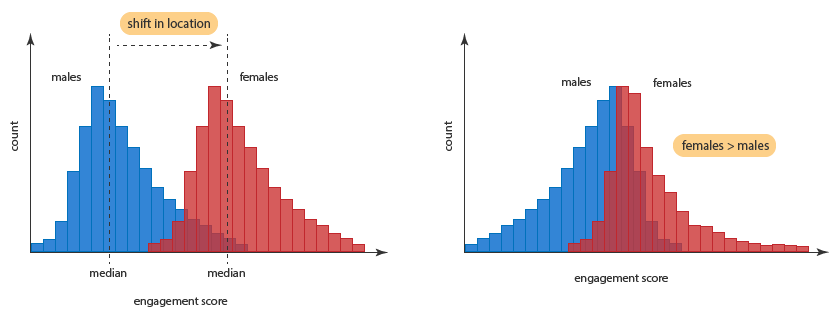
\includegraphics[width=0.6\textwidth]{figures/chapter-2/counterfactual-vs-supervised-learning.png}
	\caption{Counterfactual Inference vs. Supervised Learning}\label{fig:counterfactual-inference-vs-supervised-learning}   
\end{wrapfigure}


The problem requires making inferences on a set of counterfactual samples using a set of factual
samples. These two quantities, however, normally do not follow the same probability distribution. In fact, this would only be the case if the treatment was assigned randomly with an equal chance of $p = 0.5$ for which we could treat the problem as a supervised learning problem.  In reality, the treatment assignment is not random but reflects a particular domain-specific policy (see section \ref{sec:propensity-score}). 

%Consider the following example illustrated in figure \ref{fig:counterfactual-inference-vs-supervised-learning}: A doctor is treating patients with ... 
% CRITICAL!!! GRAPH Write proper example that corresponds with figure
%For example, one may be interested to know the consequences of smoking or the consequences of going to university. The people 'treated' are simply those—the smokers, or the university graduates—who in the course of everyday life undergo whatever it is that is being studied by the researcher. In both of these cases it is unfeasible (and perhaps unethical) to randomly assign people to smoking or a university education, so observational studies are required. The treatment effect estimated by simply comparing a particular outcome—rate of cancer or lifetime earnings—between those who smoked and did not smoke or attended university and did not attend university would be biased by any factors that predict smoking or university attendance, respectively. PSM attempts to control for these differences to make the groups receiving treatment and not-treatment more comparable. (WIKIPEDIA)

Formally, we are inferring the outcomes over a counterfactual dataset $CF = \{(x_i, 1 - t_i) \}^{n}_{i=1}$ which is distributed according to some probability distribution $CF \sim P^{CF}$ using outcomes that were estimated over a factual dataset $F = \{(x_i, t_i) \}^{n}_{i=1}$ with $F \sim P^{F}$ where $P^{CF} \neq P^F$. We are a dealing with a \emph{covariate shift} which is often encountered in domain adaptation problems (\cite{domain-adaptation}).

Consequently, if we simply treated the treatment assignment as an ordinary input feature in our dataset, we might be introducing significant biases caused by the covariate shift.  Therefore, it can be said that when performing counterfactual inference, we have to take specific measures in order to ensure a meaningful estimation of the ITE that overcomes the covariate shift problem caused by the selection bias of the treatment assignment. 


\subsection{Treatment Assignment and Propensity Score} \label{sec:propensity-score}
Whether or not a context receives the intervention typically depends on an underlying domain-specific policy. Such policies can be well-defined in  a rule-based setting like 
\begin{equation}
\text{age}(x) < 45 \wedge \text{HIV}(x) = \text{negative} \rightarrow T_x = 0
\end{equation} 
or less rigorous and simply reflect a decision maker's informal intuition. In both cases, it is important to understand that -- even though we might not be able to comprehend the policy -- the decision is not made randomly but depending on the concrete features of the context or subject. 

In the scope of counterfactual inference, we typically do not assume any kind of control or knowledge of the policy. Instead, we model a subject's inclination to receive the treatment as a random variable called \emph{propensity score} defined as 

\begin{equation}
p(x) = \mathbb{P}(W_i = 1 \mid X_i = x)
\end{equation}
where $X_i$ denotes the subject's features and $W_i$ the treatment assignment with $W_i \not \perp X_i$ (the treatment assignment is not independent from the features). 

While the propensity score is defined for each subject individually, we are sometimes also interested in the \emph{average propensity score} 

% TODO Is this the same as average treatment assignment? 
\begin{equation}
	\mathbf{B} = \frac{1}{n} \cdot \sum \limits_{{i=1}}^{n}  \mathbb{P}(W_i = 1 \mid X_i)
\end{equation}

for a given dataset yielding an estimate of the selection bias of the policy. 

\subsection{Estimating Treatment Effects} \label{sec:status-quo}
% TODO Check out Ahmed's related work sections
A number of different methods and models has been proposed in order to estimate treatment effects. 

\paragraph{Propensity Score Matching} Early works were not able to estimate the ITE directly but focuses on the \emph{average treatment effect} or ATE instead, defined as the expected value of all individualised treatment effects

\begin{equation}
\text{ATE} = \mathbb{E}[T(x)]
\end{equation}
over a population of interest using a method called \emph{propensity matching}. % CITE propensity matching (Rubin, 2011; Austin, 2011; Abadie & Imbens, 2016; Rosenbaum & Rubin, 1983; Rubin, 1973).

Propensity score matching  can be summarised as follows: First, we estimate the propensity scores of each subject in the dataset. This is achieved by training a classifier, typically logistic regression or random forests, on the dataset using the treatment assignment as target value that we want to predict. Secondly, we match each subject in the control group (i.e. the subset of untreated patients in the dataset) to one or more (e.g. by using k-nearest-neighbour) corresponding subjects in the treatment group that most closely resemble the untreated subject. Finally, we are able to estimate  the average treatment effect by computing the average of the differences between the matched subjects. 

However, it has been pointed out (\cite{propensity-score-matching-sucks}) that there are a number of limitations and challenges for this approach. For instance, in a randomised trial (i.e. $p =0.5$) the propensity scores of any two subjects will roughly be equal while their features can be significantly different resulting in misleading predictions. (\cite{propensity-score-matching-sucks}) goes as far as saying that propensity scores should not be used for matching at all. 

In addition, propensity score matching is limited to estimating the \emph{average }treatment affect and does not allow us to compute the more fine-grained ITE. 


% Classical works have focused on estimating “aver- age” treatment effects through variants of propensity score matching (Rubin, 2011; Austin, 2011; Abadie & Imbens, 2016; Rosenbaum & Rubin, 1983; Rubin, 1973). More recent works tackled the problem of estimating “indi- vidualized” treatment effects using representation learn- ing (Johansson et al., 2016; Shalit et al., 2017), Bayesian inference (Hill, 2012), and standard supervised learning (Wager & Athey, 2015).
%

\paragraph{Direct Modelling}
Despite the differences of counterfactual inference to supervised learning, it has been attempted model the ITE directly for instance using K-nearest-neighbour matching, or more recently using random forests (\cite{random-forests}) and neural networks (\cite{sontag-direct-modelling}) that are treating the treatment assignment as a feature.

One way to address the problem of covariate shift caused by the selection bias described in section \ref{sec:cfi-vs-supervised-learning}, is to introduce a dedicated term in the objective function that penalises the imbalance between the factual and counterfactual distributions.  


\paragraph{Representation Learning} \label{sec:representation-learning}
Most recently, deep neural networks have been applied to the problem of counterfactual inference resulting in promising first results. 

One of the current state-of-the-art methods called \emph{balancing neural network} (BNN) treats the task as a problem in \emph{representation learning} (\cite{sontag-paper}).

The approach is based on the concept of learning balanced representations for the treated and untreated subjects in the dataset such that the discrepancy between the distributions of the factual and counterfactual outcomes is reduced. 

\begin{figure}[h]
	\centering
	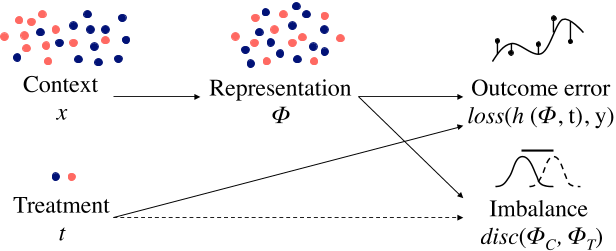
\includegraphics[width=0.8\textwidth]{figures/chapter-2/balanced-representations.png}
	\caption{Learning Balanced Representation for Counterfactual Inference}\label{fig:balanced-representations}
\end{figure}

Concretely, they propose an architecture for feed-forward neural networks (illustrated in figure \ref{fig:balanced-representations-architecture}) in which the first $d_r$ hidden layers are responsible for learning a balanced representation $\Phi$ which is then processed in the remaining $d_o$ hidden outcome layers. 
The imbalance of the representation is minimised in terms of a function \emph{disc} whereas the outcome is optimised using the objective function 

\begin{equation}
	\text{loss}(h(\Phi, t), y) = \frac{1}{n}\sum_{i=1}^{n} \mid h(\Phi(x_i)), t_i), - y_i^{F} \mid
\end{equation}

that computes the absolute error between the prediction of the learnt hypothesis function $h$ on the inputs $x_i$ represented in terms of the learnt representation $\Phi$ and the actual (factual) outcome $y_i^F$. 

\begin{figure}[h]
	\centering
	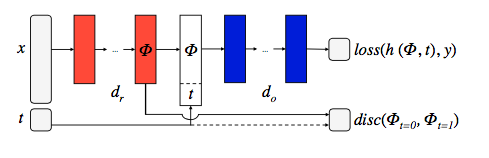
\includegraphics[width=0.8\textwidth]{figures/chapter-2/sontag-architecture.png}
	\caption{Architecture for Balanced Representations}\label{fig:balanced-representations-architecture}
\end{figure}

Their method consistently outperformed competing approaches and can be considered state-of-the-art. 


\paragraph{Deep Neural Networks} 
Despite the recent successes of deep neural networks in many problem areas, only limited research has been done on using them for the task of causal inference. However, the previous example of representation learning \cite{sontag-paper}, indicates promising first results and demonstrates that neural networks can be highly suitable for the task. 
 
This thesis deals with the questions of how to improve the state-of-the-art in counterfactual inference using deep neural networks. In the following chapters, we propose a novel architecture for neural networks that conceptualises the problem as a multi-task learning problem, we introduce a propensity-based dropout scheme for regularisation and overcoming the selection bias, and present an efficient way to infer suitable hyper-parameters for the model. 


%\subsection{Challenges}
%How to improve accuracy? 
%What are good architectures? 
%How to train them? 
%Dropout? 

